\documentclass[a4paper,twocolumn]{esapub2005} % European paper
\pagestyle{empty}

% introduce this option for the ESA publications style
\bibliographystyle{unsrt}

\usepackage{times}
\usepackage{natbib}
\usepackage{graphicx}
\usepackage[hyphens]{url}
\usepackage{subfig}
\usepackage{placeins}
\usepackage{float}
\usepackage{titlesec}

%\title{High performance on-board image processing using CANopen for Earth observation satellites}
\title{HIGH PERFORMANCE AND REUSABLE APPROACH TO ON-BOARD IMAGE
PROCESSING APPLIED TO EARTH OBSERVATION}

\author[1]{Yago Isasi Parache \thanks{isasi@luxspace.lu}}

\affil{LuxSpace S\`arl, Luxembourg}
\author[2]{Dr. Pablo Ghiglino \thanks{ pablo.ghiglino@klepsydra.org}}
\affil{Klepsydra Robotics, GmbH. Zurich, Switzerland}

\author[1]{Nicolas Perzo \thanks{perzo@luxspace.lu}}


\newcommand{\btx}{\textsc{Bib}\TeX}
\newcommand{\filename}{esapub}


\titlespacing\section{0pt}{10pt plus 2pt minus 1pt}{0pt plus 1pt minus 1pt}
\titlespacing\subsection{0pt}{10pt plus 2pt minus 1pt}{0pt plus 1pt minus 1pt}
\titlespacing\subsubsection{0pt}{10pt plus 2pt minus 1pt}{0pt plus 1pt minus 1pt}

\begin{document}
\maketitle
\keywords {OBDH, OBDP, Earth Observation, CAN-BUS CANopen, flight software}
\begin{abstract}
Earth observation (EO) has been and still is a very complex topic in the Space Engineering field. Yet there is a growing number of new requirements and needs for new EO nano and microsatellites, working either standalone or in synchronized constellations. Higher download data rates, improved image quality and enhanced onboard computing capabilities are only a few examples of the challenges to be faced in this discipline. Furthermore, the need to speed up the time to market and reduce costs of development, has sparkled the use of modular solutions over monolithic ones for payload computer design, where purpose specific components - hardware and software - are reused and assembled for different spacecrafts and missions. In this work, we present a modular approach to on-board image processing based on a distributed computing setup with functionality specific computers connected to an on-board CAN-BUS using CANopen protocol. Optimal use of the resources in the network is achieved by a two-fold design consisting in using FPGAs for data processing and compression and in integrating a high performance software library data handling and data communications. The feasibility of this approach is tested in a two-node network for an EO payload with an image capture and compress node and an Earth Link node. Results are presented based on image size and performance parameters. 

\end{abstract}

\section{Introduction}
\subsection{Trends of small satellites}

Since the year 2011, an increasing number of small satellites (\textless 100Kg) has been registered. In particular 70\% of the value is in the area of micro satellites in the range of 25Kg to 100Kg. According the NSR \cite{NSR_WEB}, the increasing trend of launches will continue in the following years to reach a \$630M value by 2025.

\begin{figure*}
\centering
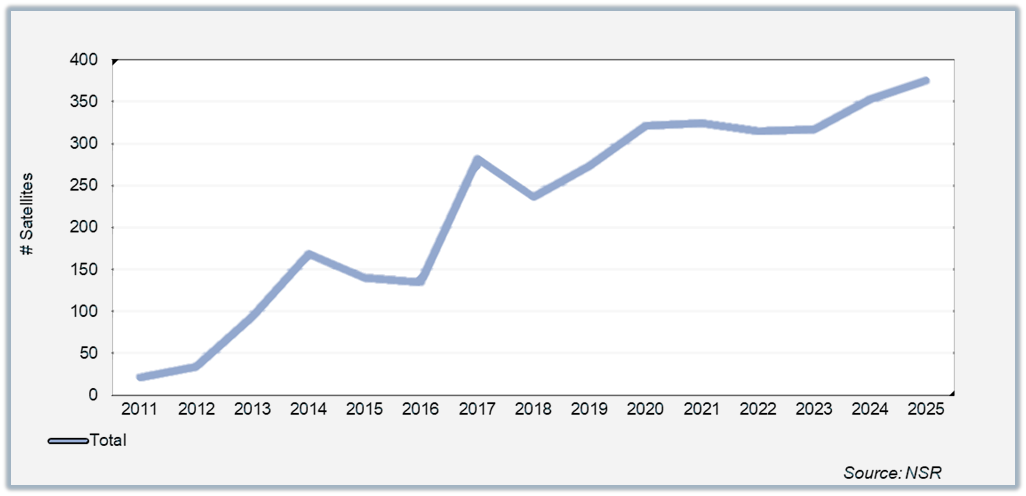
\includegraphics[width = 5in]{images/trend_small_sats}
\caption{Trend of small satellite launches from 2011 to 2025.\label{fig:single}}
\end{figure*}

While in the decade of the 80's 70\% of the small satellites where dedicated to telecommunication applications the trend seems to indicate that by 2025 Earth Observation(EO) and situation awareness applications will cope most of the satellite market.

\begin{table} [!h]
  \begin{center}
    \caption{Satellite global market payload application evolution}\vspace{1em}
    \renewcommand{\arraystretch}{1.2}
    \begin{tabular}[h]{lrcc}
      \hline
      Payloads & 1980s-1990s  &  2005 \\
      \hline
      Earth observation  & 1.4\% & 47\%\\
      Situation awareness  & 2.3\% & 10\%\\
      Communications  & 69.2\% & 12\%\\
      In-orbit Demonstrators  & 11\% & 18\%\\
      Others  & 16.1\% & 13\%\\
      \hline \\
      \end{tabular}
    \label{tab:table}
  \end{center}
\end{table}

The global commercial satellite imaging market is a large growth area, with increasing demand for high resolution imagery. The market was valued at US \$1.6Bn in 2014 and is projected to reach US\$3.5Bn by 2024 [1]. The use of CubeSats and Microsatellites in satellite imaging, particularly EO, is rapidly increasing with the small satellite EO market value expected to be US\$350M over the next six years. Sectors making use of EO satellite imagery include defence and security, insurance, disaster monitoring, agriculture, civil engineering and energy, as well as government use. Options for commercial off-the-shelf imaging systems that fit for a wide range of EO, are more and more available for satellite integrators to purchase and integrate into a satellite. It is also true, that the market is not fully developed yet at lower costs.

\subsection{CAN in space}
 The controller area network (CAN) protocol is a highly reliable communication system for harsh environments and has been used in automotive and industrial applications since its presentation in 1986. The CAN two-wire bus multi-master/multi-drop topology makes it easy to add additional functionality to a system while significantly reducing the number of wires associated with the wire intensive point-to-point topologies used in the past. The space community was aware of the CAN protocol’s many benefits and advantages, and the need for it to replace traditional spacecraft bus architectures, however CAN was not fully used in space systems. With the emergence of of the QML-V qualified radiation tolerant CAN-Bus transceivers \cite{COBHAM}, and the qualification of several CAN-enable rad hard microcontrollers, design and implementing a CAN bus network for spacecraft on-board communications with the characteristics and benefits of terrestrial CAN-based embedded system is perfectly possible. The use of CAN-Bus for internal communications onboard spacecraft is becoming more and more common ground. The general use of CAN-Bus communication in spacecrafts is shown in e.g. \cite{CANBUS1}, The use of CAN-Bus in CubeSats is presented in \cite{CANBUS2}. Furthermore, CANopen protocol is also used extensively in space. \cite{RENESAS_CAN_Open} presents the industrial use of CAN-open in space. More importantly, \cite{ESA_CAN_Open} is the official specification provided by ESA for CANopen for onboard communications.

\subsection{CANopen at LuxSpace}
At LuxSpace the use of CAN-Bus systems was introduced during the development of the E-SAIL project. It has allowed engineers to replace older architectures with more complex wiring communications, with a CAN two-wire bus network. Reducing the number of wires and weight along with lower power consumption and easier testability that resulted in important cost savings due to the easier testability. In particular, during the design, implementation and testing of the E-SAIL project, we used a tailored implementation of the ECSS-E-ST-50-15C standard. LuxSpace vision was to reuse the existing and well proven parts of CANopen, as needed by the E-SAIL project, removing the parts which were not explicitly required. Comparing networks in the automotive and space domains, in a typical CAN network in an automotive environment a big advantage of CANopen is that device profiles exist and nodes can be easily replaced by products from other manufacturers. Each node, sharing the same device profile, provides a set of functions to identify it and configure it online to exchange information with the existing network. This allows to be very flexible and agile when setting up new networks. In the case of space, the network is well defined and all nodes and most parameters are known a priori. Moreover, the replacement of nodes after launch is indeed not possible. In E-SAIL, that was exactly the case, having a physical architecture based on a multi-drop topology, with two independent buses; one nominal and one redundant. Only one bus is active at a time (cold redundancy). The bus ends are terminated external to the units in order to allow flexibility for the arrangement of the unit. ISO11898-2:2003 transceivers have been used for both nominal and redundant bus. Additionally, Several tools and methods commonly used by automotive industry in design, development, production and maintenance of CAN bus networks for safety critical applications have been used successfully used during the implementation and testing of E-SAIL, as the CANoe tool. As a direct result of the E-SAIL development, the CANOpen modules developed in the frame of the project are expected to be reused as libraries in the future microsatellite projects in the company. Due to the market explosion on EO and Situation awareness satellites, it was necessary to step forward on extending the use-cases covered by the E-SAIL project. LuxSpace worked with Klepsydra on novel modular approach to on-board image processing based on a distributed computing setup with functionality specific computers connected to an on-board CAN-Bus using CANopen protocol. The performance of the network solution is a critical aspect for the future platform at LuxSpace, specially when high volumes of data will need to be processed through it. The following sections describe the system, the software design and the results of our study where optimal use of the hardware resources in the network is achieved by, from one side using FPGAs for data processing and compression and by integrating the Klepsydra software, a high-performance software library for data handling and data communications.

\section{System Design}

Several works that show the advantages of using a distributed architectures. For example, ~\cite{DIST_COMP1} presents a distributed architecture for small satellites, ~\cite{DIST_COMP2} presents a fault-tolerance solution based on distributed architectures.  One of the current trends in the onboard computer design, is the use of small boards that host a FPGA. Example of the use of this approach can be found in \cite{FPGA1} and \cite{FPGA2}. For our particular system we have selected a Zynq Board, that is attracting some interest by its cost and extended features, in particular the support for CAN. \cite{NASA_ZYNQ} has already made some experiments with this board in the ISS. Also, \cite{VIS_NAV1} proposes a visual navigation solution based in the Zynq board. 

In regards to image compression, most solutions for Earth Observation are based in discrete wavelet transform (DWT). \cite{DWT1}, \cite{DWT2}, \cite{DWT3}, and \cite{DWT4} are research work in this type of compression applied to satellites. Furthermore, \cite{ESA_DWT} provides this specification for DWT compression applied to Earth Observation and also \cite{ESA_FPGA} presents an implementation of DWT for FPGA. 

Luxspace and Klepsydra decided to work on a distributed architecture that could be used in the frame of EO projects. The solution proposes a two-node solution, with one computer connected to the camera and performing capturing and compressing, and the second node that receive the image via CAN-Bus and send it to Earth. In our system, both nodes are Zynq boards.

\begin{figure}[!h]
\centering
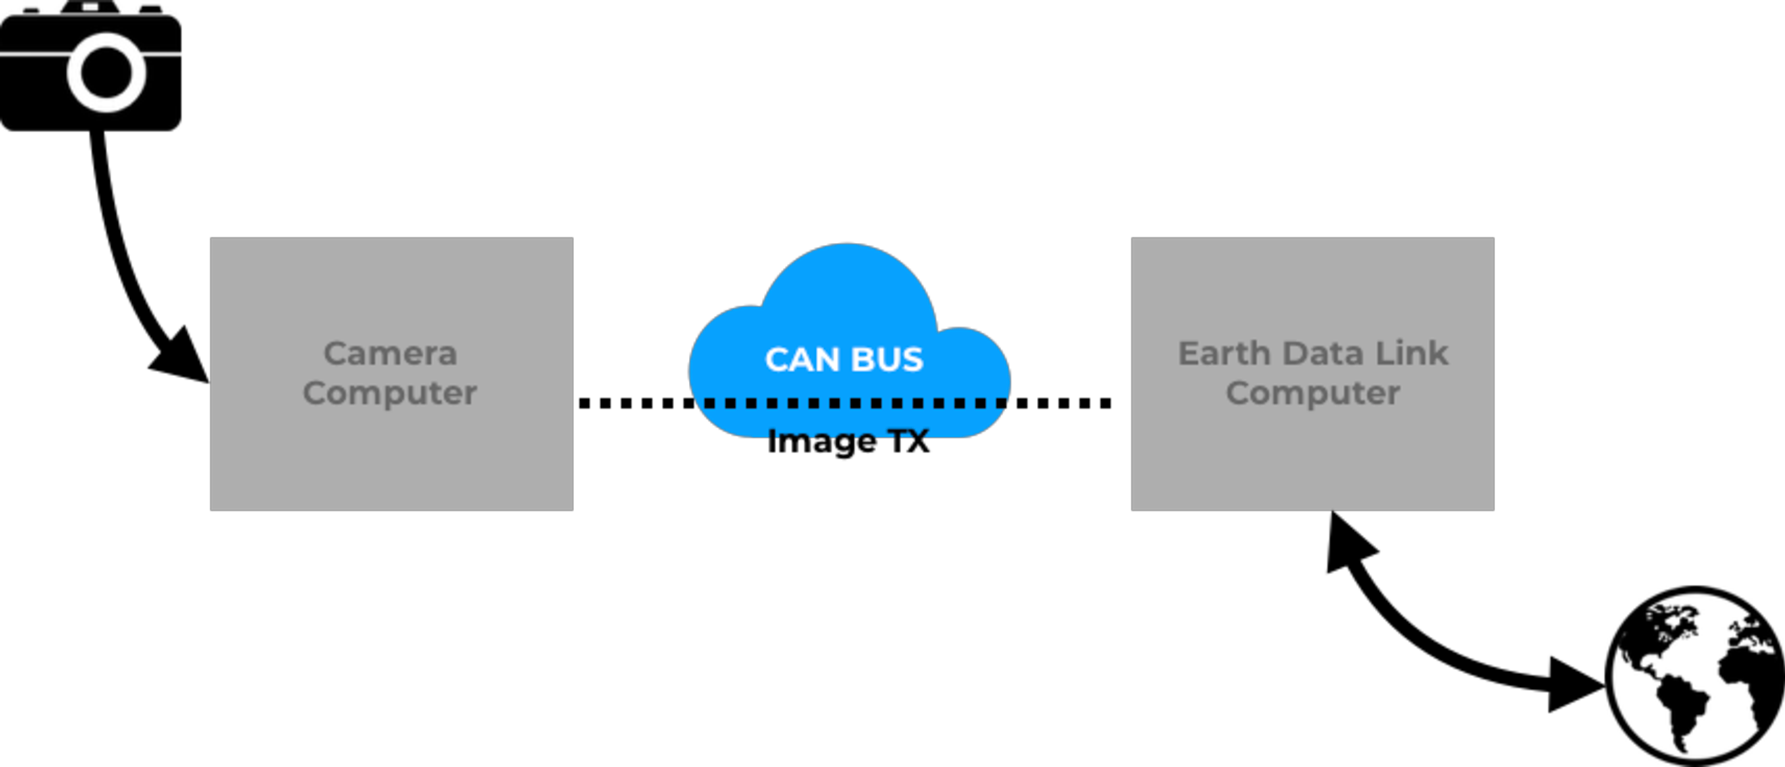
\includegraphics[width = 3in]{images/distributed_architecture}
\caption{Distributed Earth Observation architecture.\label{fig:distributed_architecture}}
\end{figure}

\section{Software Design}

In terms of SW, the different layers are described in Figure ~\ref{fig:canopen_img_tx_protocol2} . from one side one node acts as a server application in charge of capturing the image, compressing it and transmitting it thought the CAN Bus. The image compression is performed in the FPGA. On the other side the client side receives the image though the CAN-Bus and downlinks to ground.

\begin{figure} [!h]
\centering
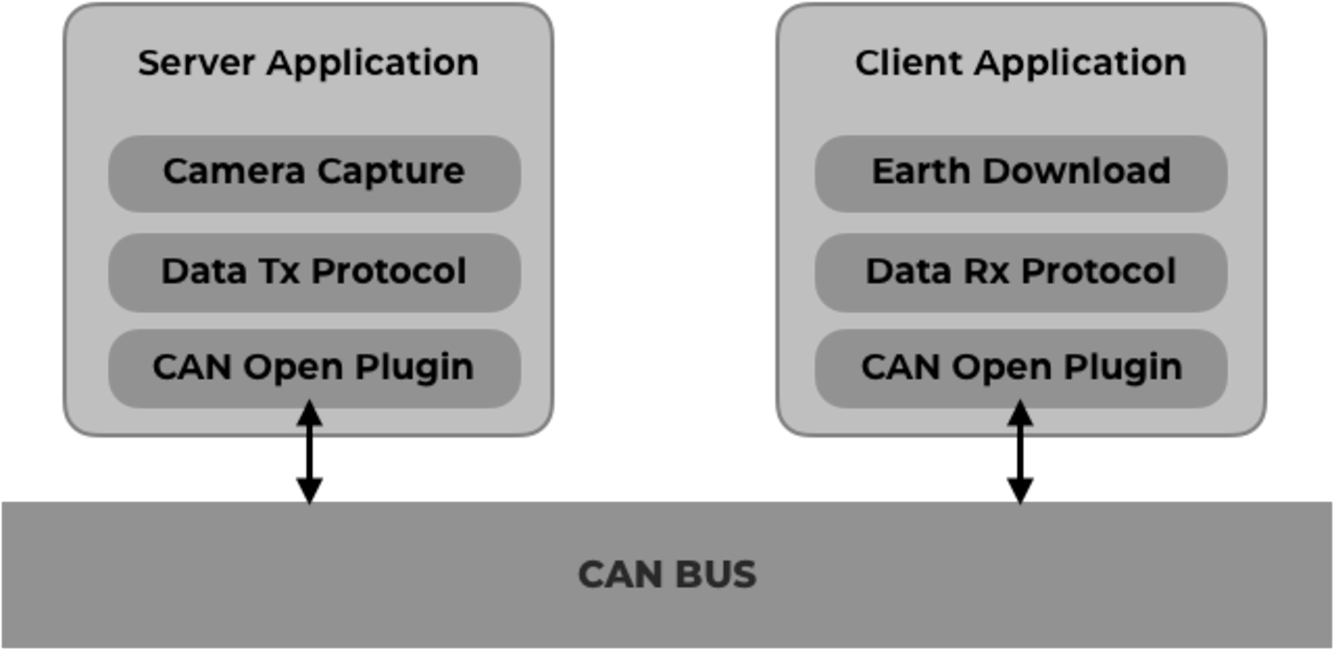
\includegraphics[width = 3in]{images/canopen_img_tx_protocol2}
\caption{Software layer design.\label{fig:canopen_img_tx_protocol2}}
\end{figure}

More is detail, the proposed solution has the following features:

\begin{itemize}
\item DWT is used for image compression. In particular, we used CCSDS 122.0 and CCSDS 123.0 
\item CANopen as communication protocol to send the image from the camera node to the Earth data link node.
\item Klepsydra Space Software.
\end{itemize}

\subsection{Klepsydra}
The solution uses Klepsydra Space, a high performance software toolset for space flight software and payload solutions. Klepsydra is a test driven, agile oriented and event-driven software, features used in the big technology companies (Netflix, Google, Amazon, etc) but also in the investment banking and electronic trading sectors. The main features of the Klepsydra software are:

\begin{itemize}
\item High performance and resource optimisation.
\item Platform independent, high level and lightweight.
\item User friendly and easy APIs.
\end{itemize}

\begin{figure}[!h]
\centering
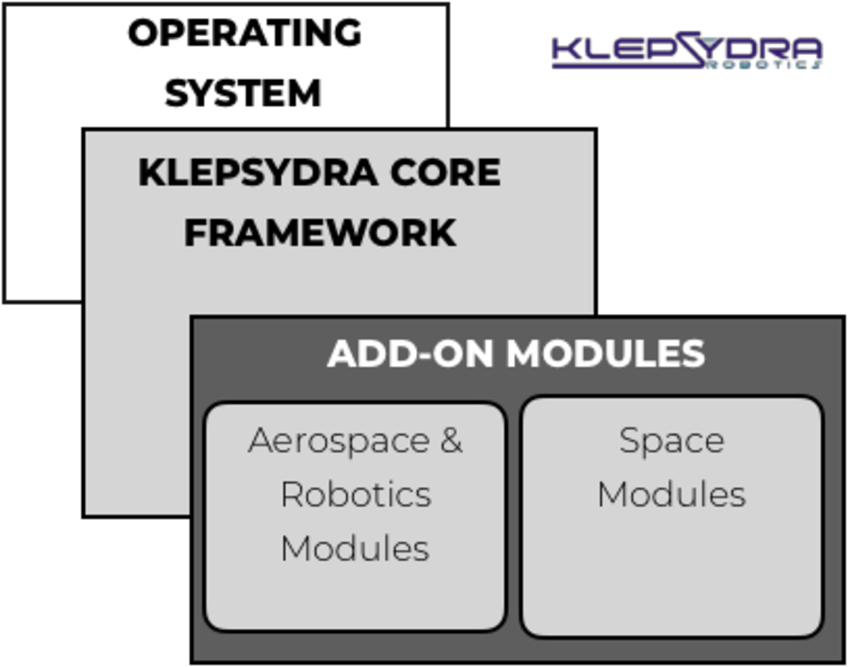
\includegraphics[width = 2in]{images/klepsydra_overview}
\caption{Klepsydra toolset overview\label{fig:kpsr_over}}
\end{figure}

We have made use of the following features of Klepsydra:

\begin{itemize}
\item kpsr-core. High performance core library.
\item kpsr-canopen. CANopen protocol connector.
\item kpsr-admin. For performance monitoring.
\item Custom module with a simple protocol for internal image transmission.
\item Control service. To start and stop Earth Observation based on critical sensor data.
\end{itemize}

\subsection{Transmission Protocol}
The custom protocol developed for this, consists of splitting the image in maximum size SDO segments (each segment is 889 SDO blocks), and using a dictionary object to control the flow that includes the Status, the number of blocks and the current block index. The statuses of the solution are NEW\_IMAGE, NEW\_BLOCK, BLOCK\_READ, LAST\_BLOCK, IMAGE\_READ. This information is all sent into one 8-byte block to save back and forth from with CAN-open. Both nodes, transmitter and received, constantly poll the CAN-open Object Dictionary for changes in the control object.

\begin{figure} [H]
\hspace*{-0.3cm}  
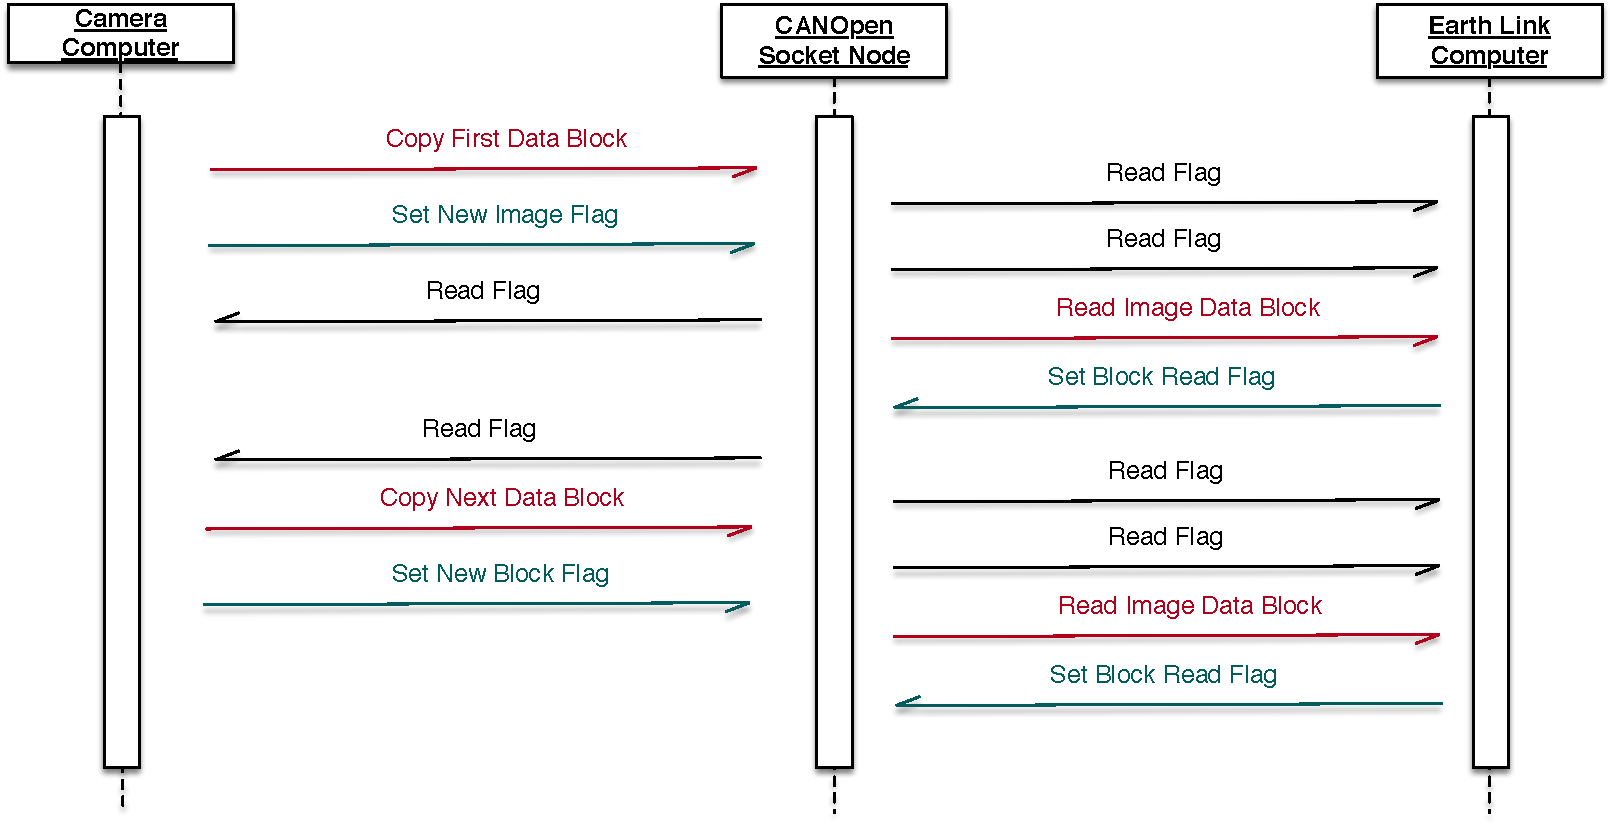
\includegraphics[width = 3.3in]{images/canopen_img_tx_protocol}
\caption{Data transmission protocol.\label{fig:canopen_img_tx_protocol}}
\end{figure}

As part of our solution, we opted for using CAN Socket combined with CANopen. CAN Socket is a convenient solution proposed by several automotive vendors to be able to share access to the CAN bus by different process running in the same processor. One of the main implementation of this specification is CANopenSocket \cite{CANopenSocket}. CANopenSocket is based on CANopenNode, which is an open source CANopen Stack. Klepsydra has developed a modified version of this implementation that makes better use of the resources and performs faster than the open source version.

\subsection{Experimental Setup}
The testing of this solution was perform in two different environments. First in Zynq boards with Petalinux \cite{PETALINUX} installed, and secondly in Zedboard with  \cite{XILLINUX} installed. The image dimensioning is: 256KB before compression and 32KB after compression. Images were transmitted with a 0.1Hz and the protocol used busy wait of 477KHz, which was the optimal rate empirically found.

\section{Results}
The results presented here are for the Petalinux setup which performs substantially better than Xilinux. The reason behind is that Petalinux is optimised for Zynq boards, while Xilinux is more oriented to development and prototyping.  The throughput of data was approximately $100$Kbps with an approximately 8\% deviation. This throughput remained constant for different sizes of images we tested on the range from 64KB to 256KB. This can be seen in figure \ref{fig:image_tx_publication_rate}.

\begin{figure}[H]
\hspace*{-0.7cm}  
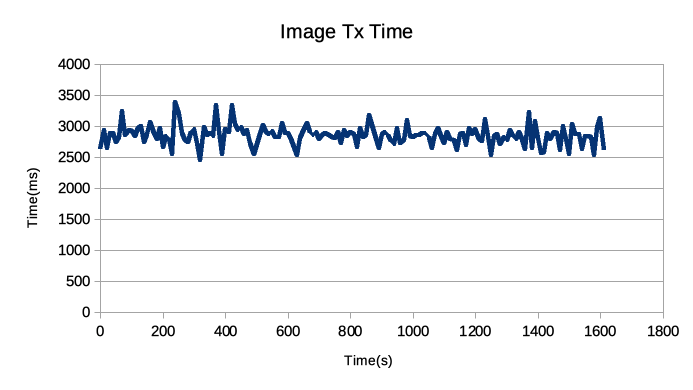
\includegraphics[width = 3.5in]{images/image_tx_publication_rate}
\caption{Image Tx Publication rate.\label{fig:image_tx_publication_rate}}
\end{figure}

This rate is roughly consistent with the CAN-Bus rate specification. CAN-open usually runs at 250 Kbps, out of which, approximately 50\% is protocol overhead. Furthermore, our custom design introduce another extra overhead of roughly 20\% depending on the busy wait rate, being finally the effective rate of 100Kbps. ($R_{effective} = 250{Kbps} \times 0.5 \times 0.8 = 100{Kbps}$).

Figures \ref{ref_label_overall} show RAM and CPU consumption for server (transmitter) and client (receiver) processes. In these figures it can be seen that the memory consumption of both processes is constant, and the CPU in both cases is limited and also roughly constant. This is due to the use of Klepsydra, which one of its best features besides resource optimisation, is its stability and predictability.

\begin{figure*}[!htbp]
  \centering
  \subfloat[Client CPU]{\label{client_cpu}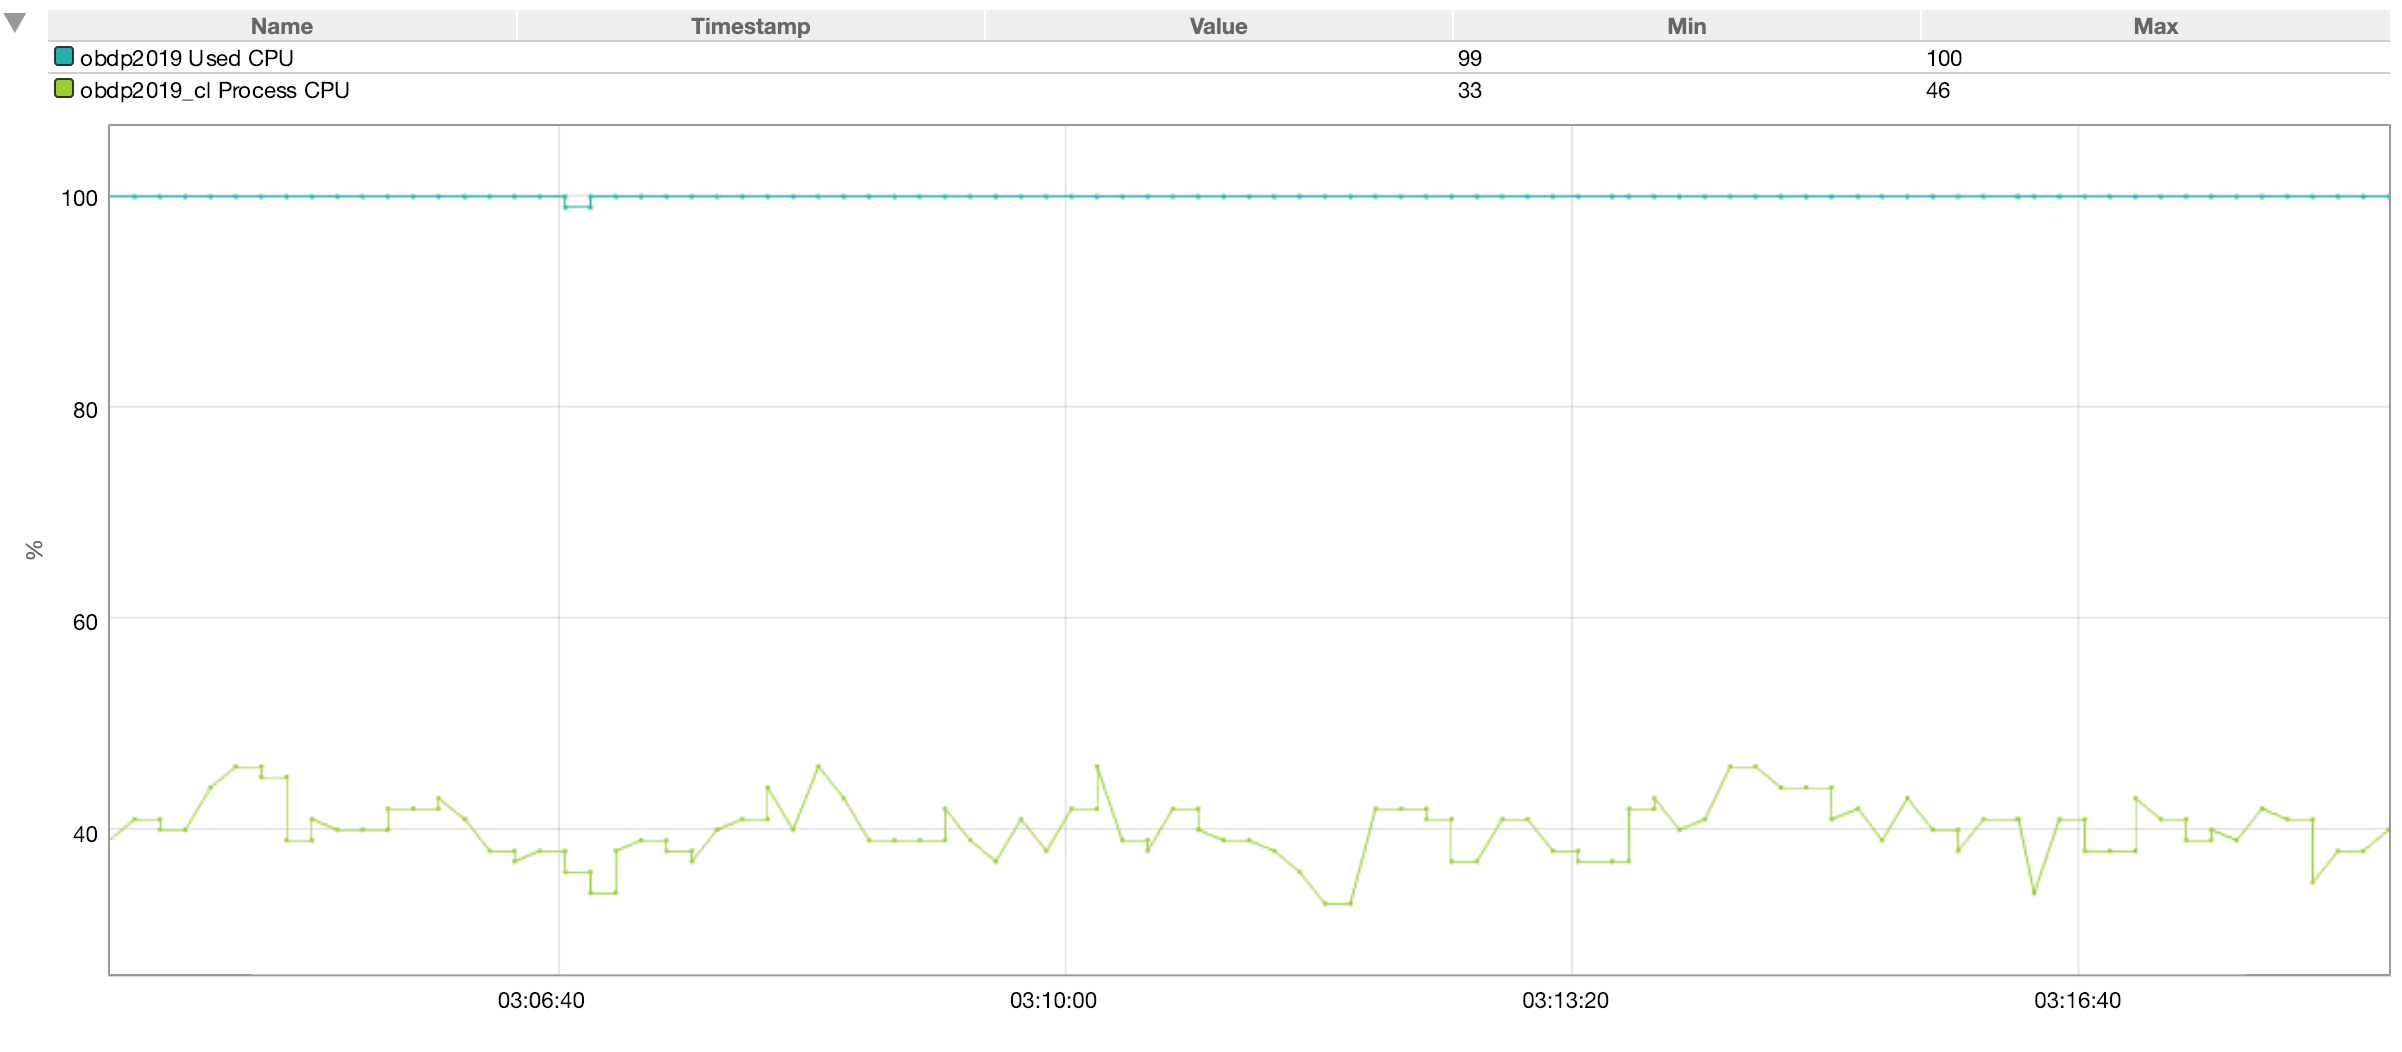
\includegraphics[width=0.5\textwidth]{images/client_cpu}}
  \subfloat[Client Memory]{\label{client_memory}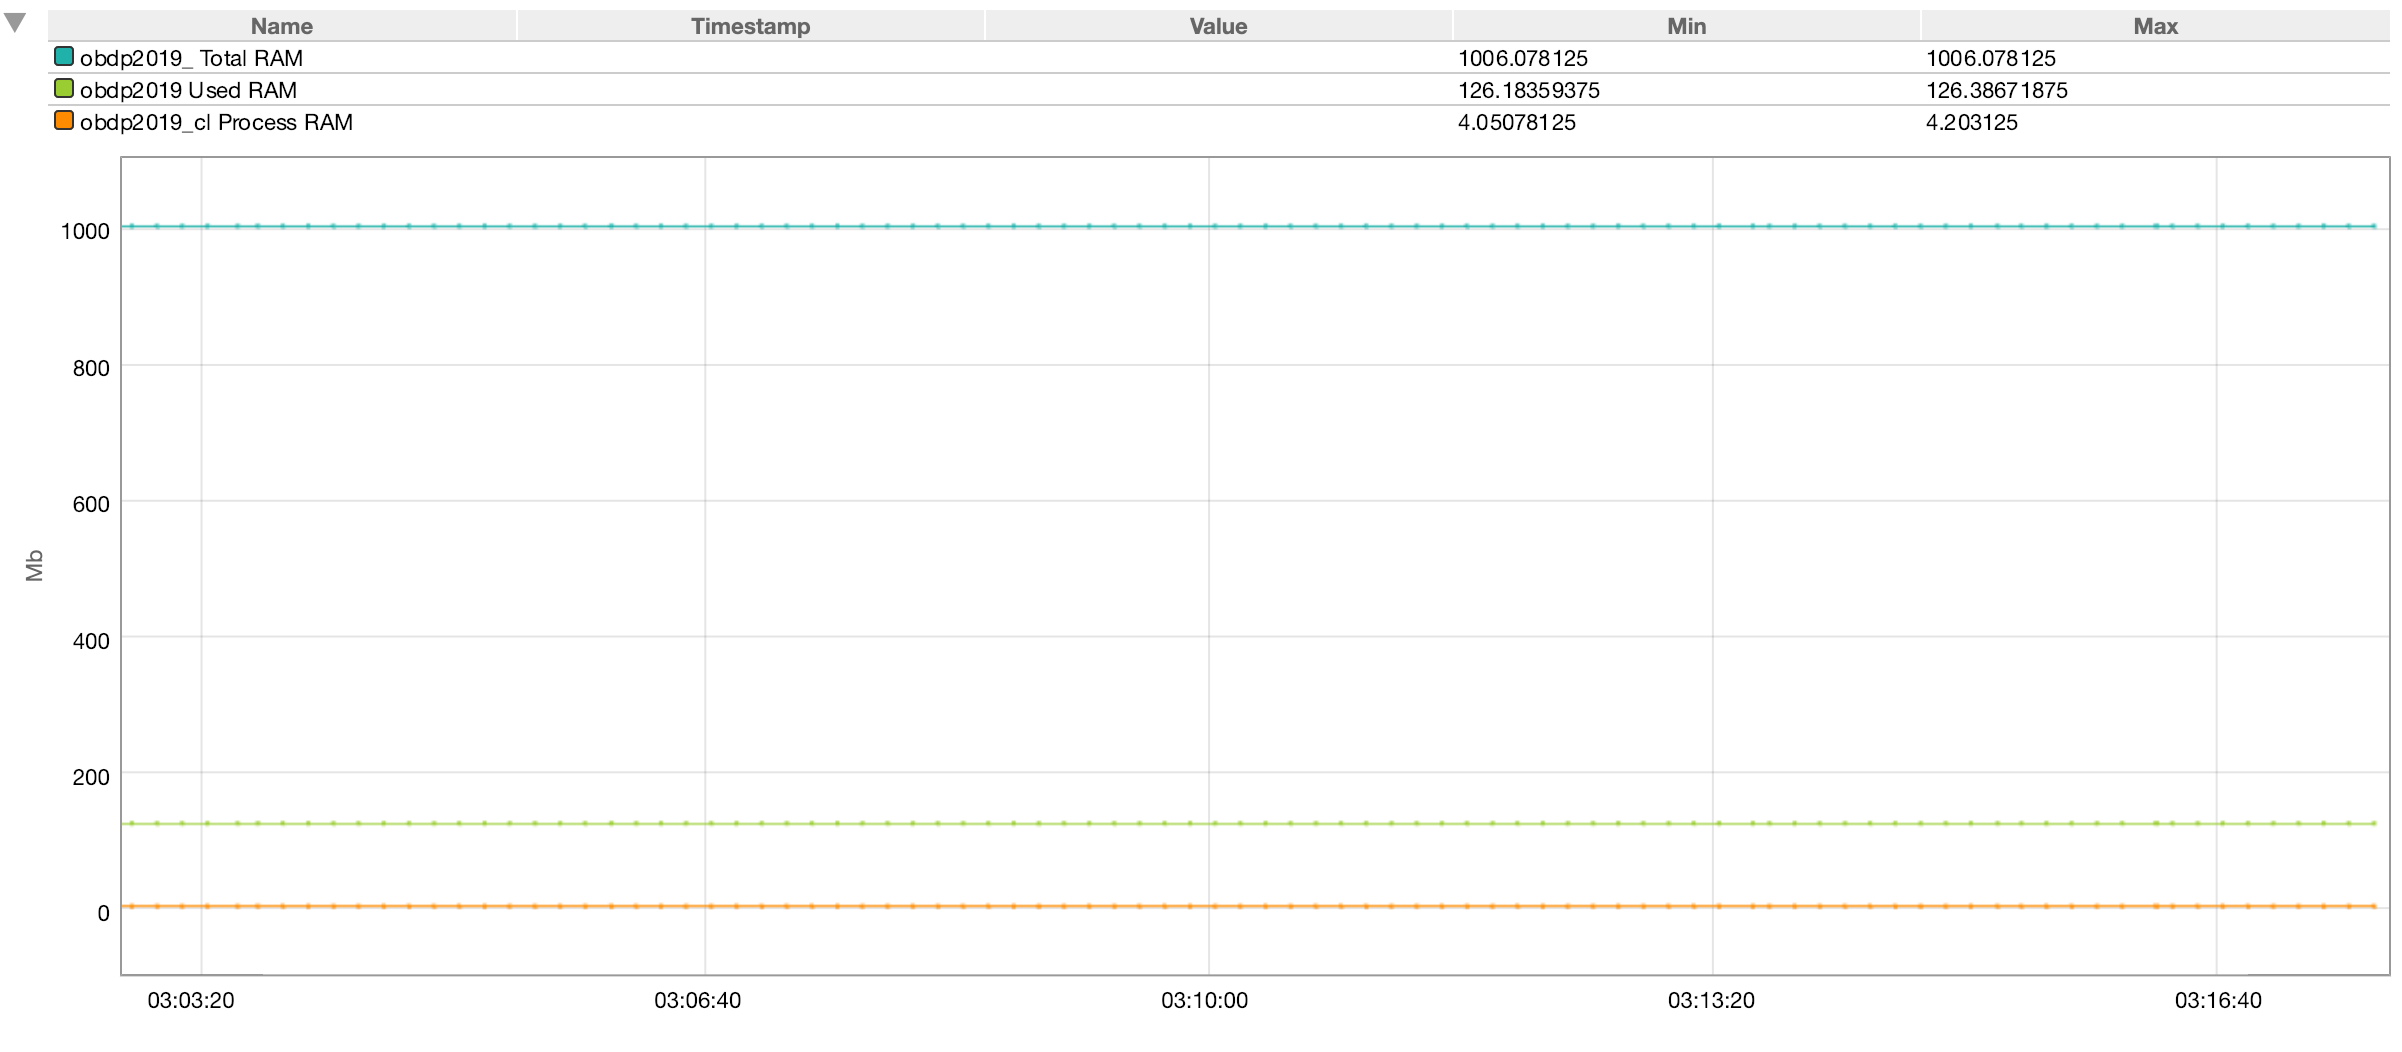
\includegraphics[width=0.5\textwidth]{images/client_memory}}\\
  \subfloat[Server CPU]{\label{server_cpu}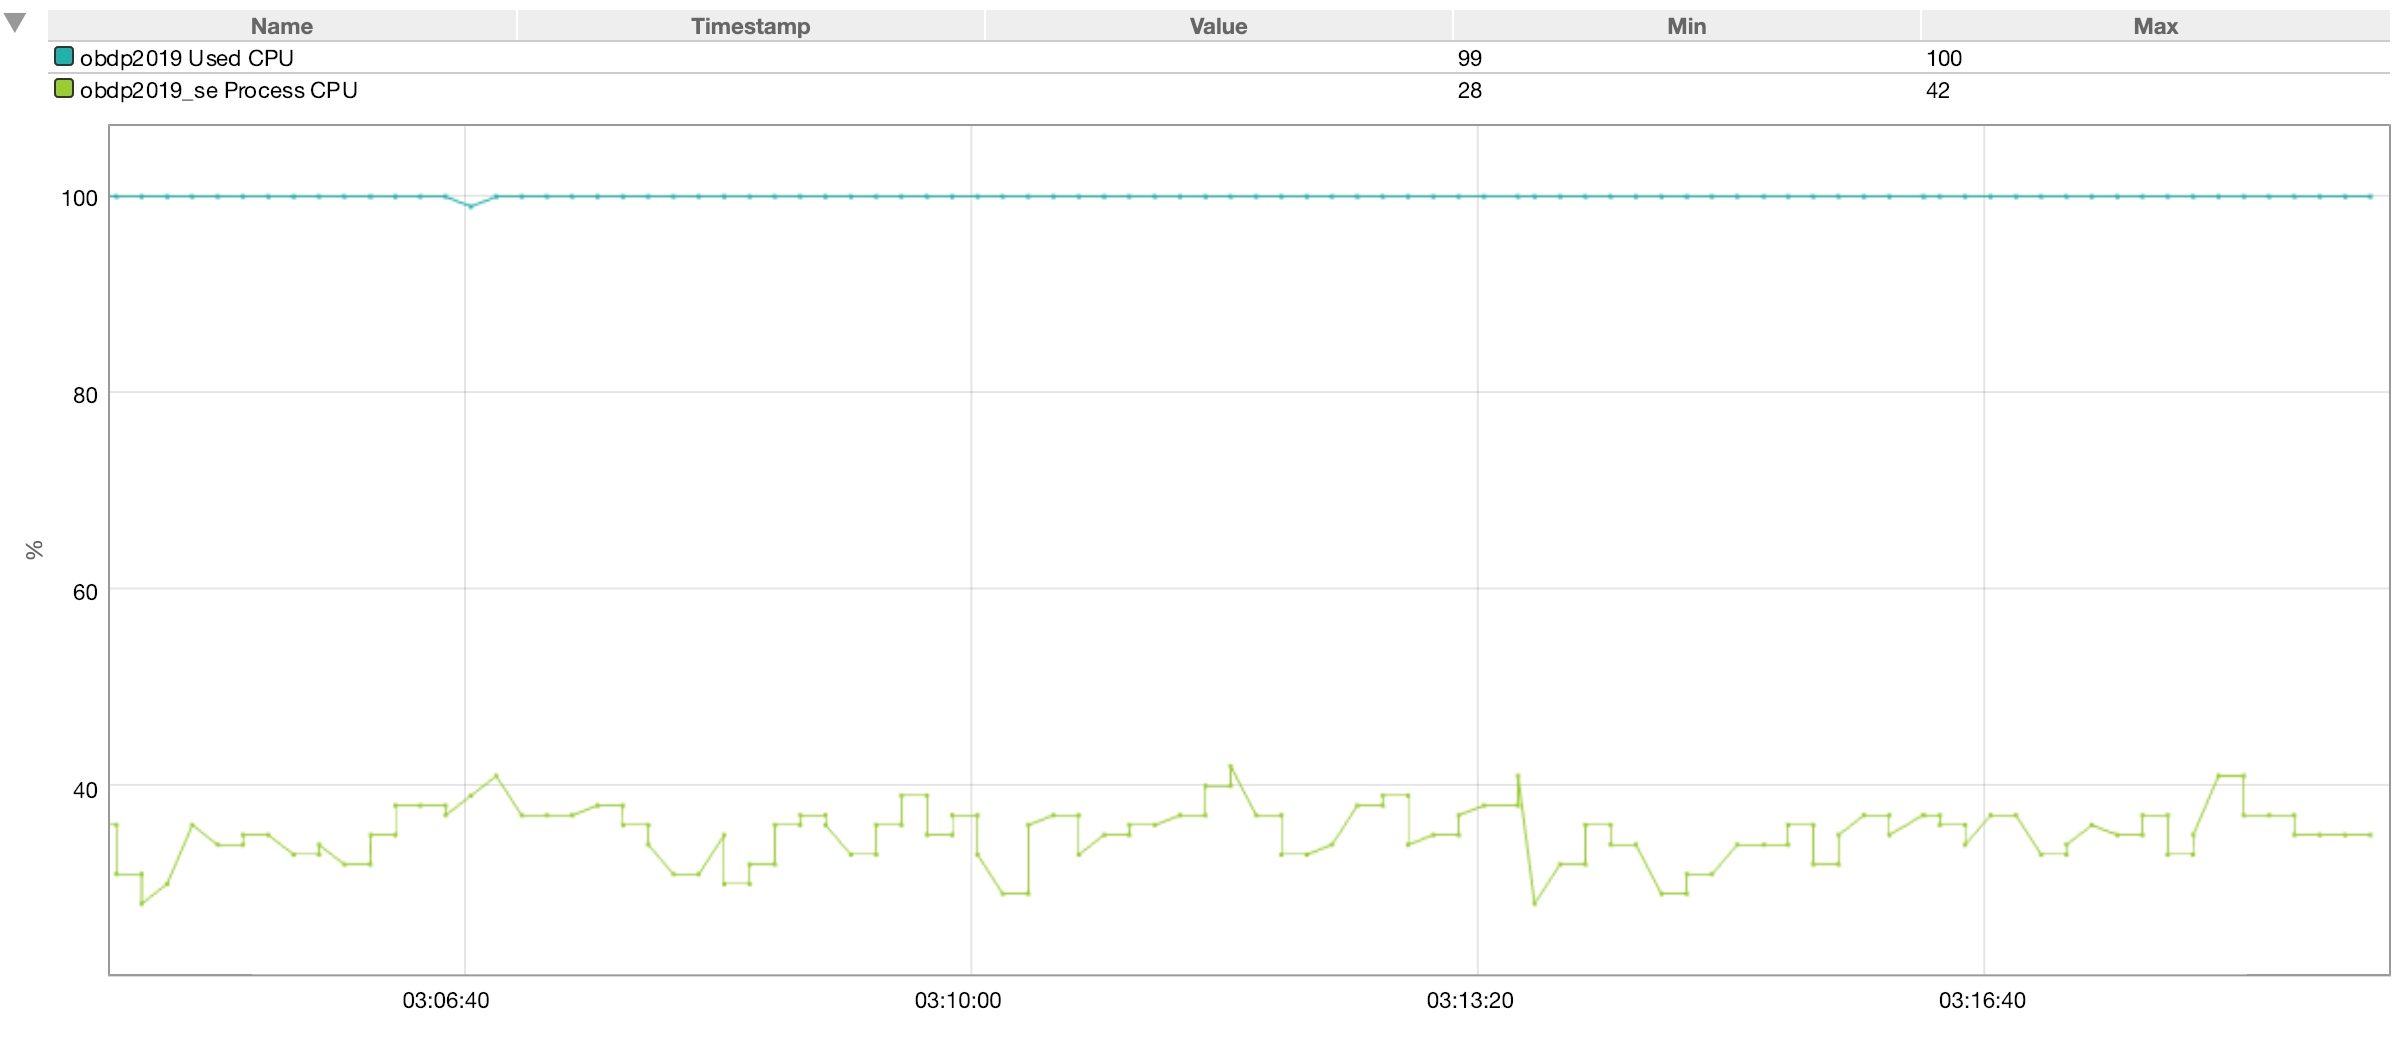
\includegraphics[width=0.5\textwidth]{images/server_cpu}}
  \subfloat[Server Memory]{\label{server_memory}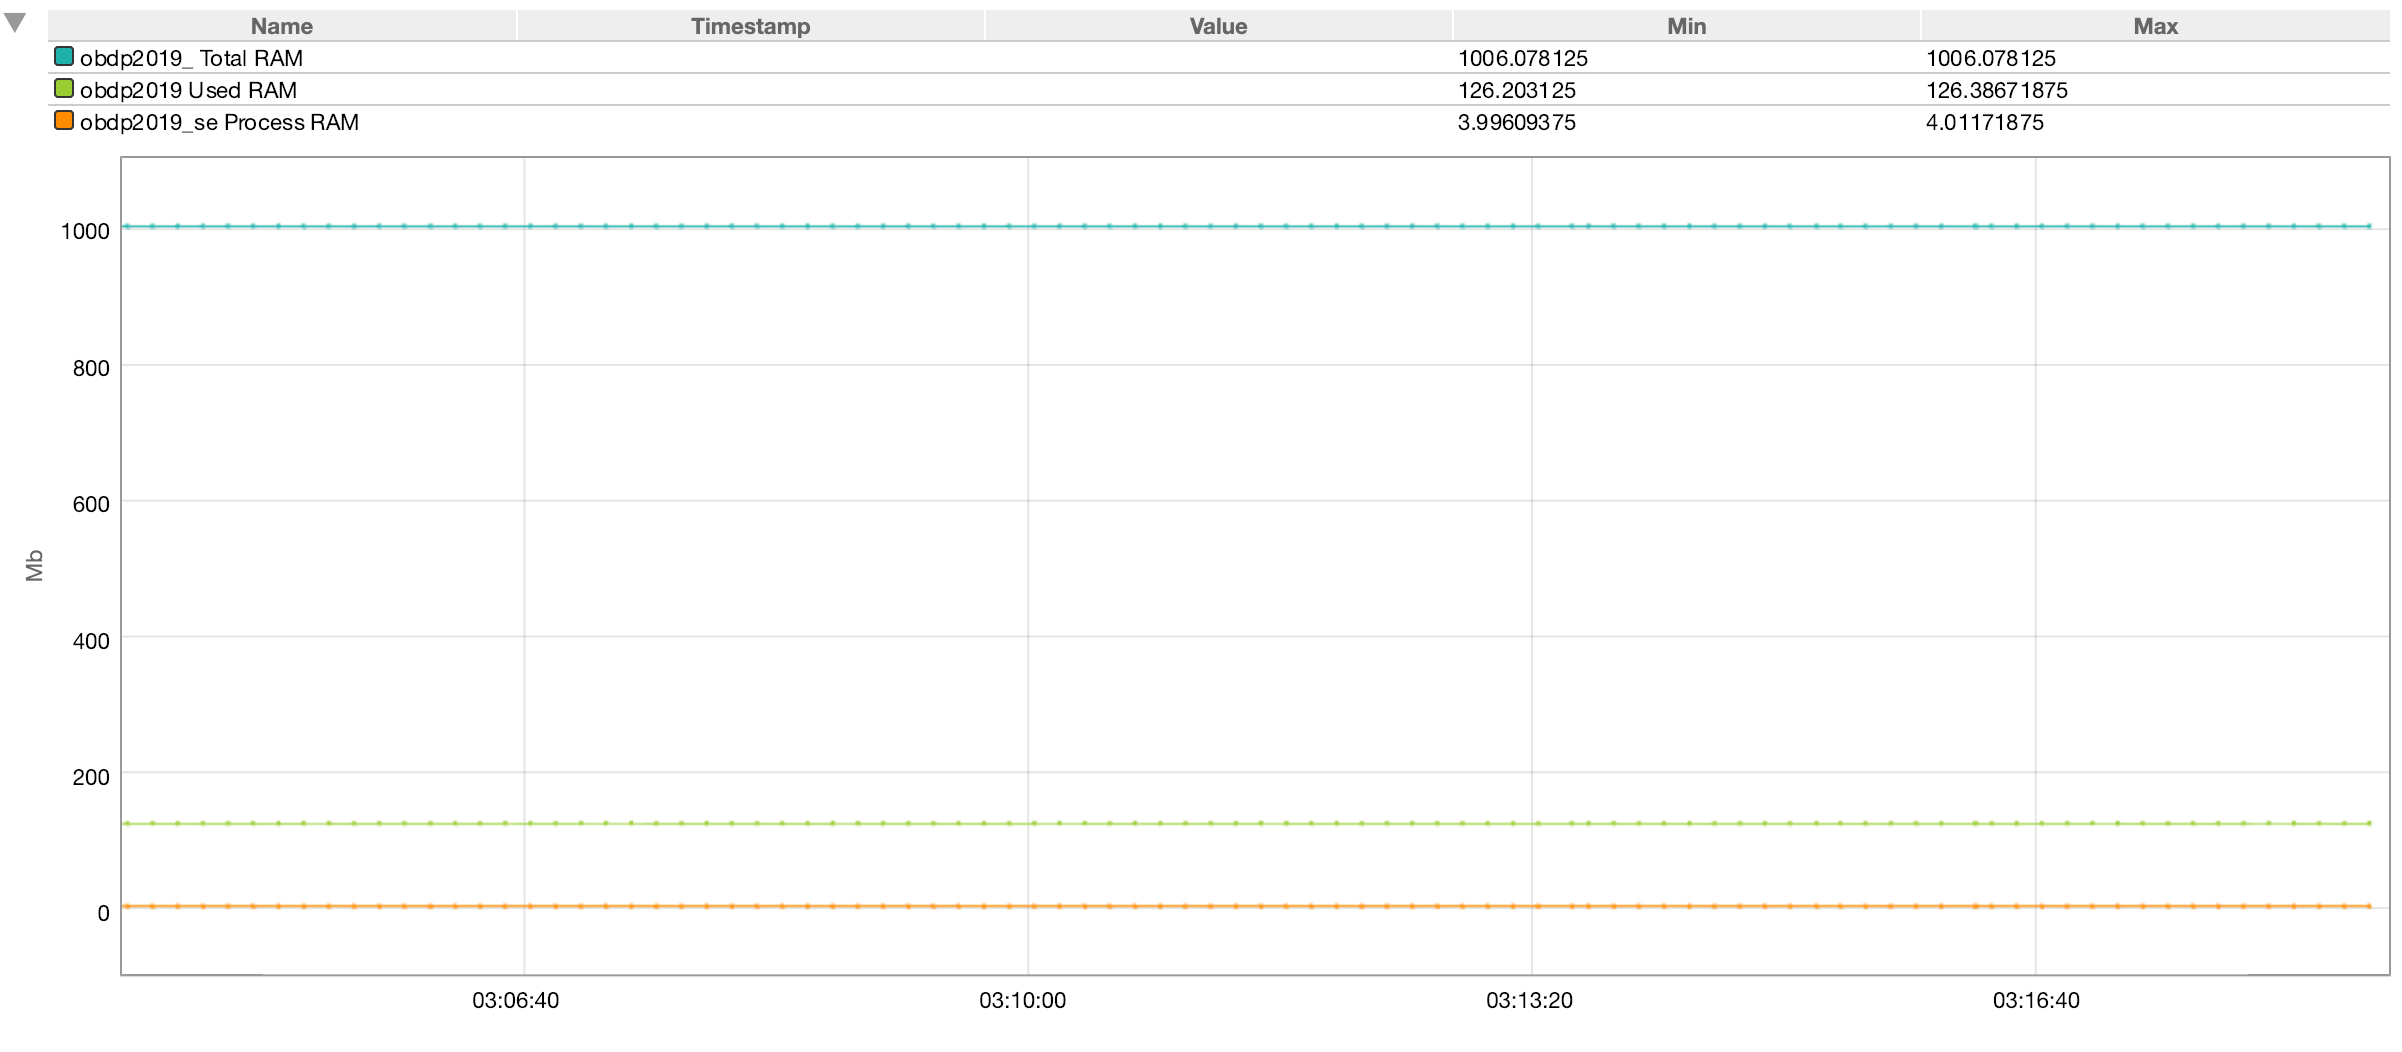
\includegraphics[width=0.5\textwidth]{images/server_memory}}
  \caption{\label{fig:ref_label_overall} Resources consumption in client and server side}
\end{figure*}

As Klepsydra bases all its usage in the publisher-subscriber pattern (\cite{Douglass2010DPEmbeddedSysinC}), in this section we show the performance of the publishers and subscribers in the client and server side. The use of busy wait can be seen to perform with great accuracy.

\begin{figure*}[!htbp]
  \centering
  \subfloat[Client Publication Rate]{\label{client_pub_rate}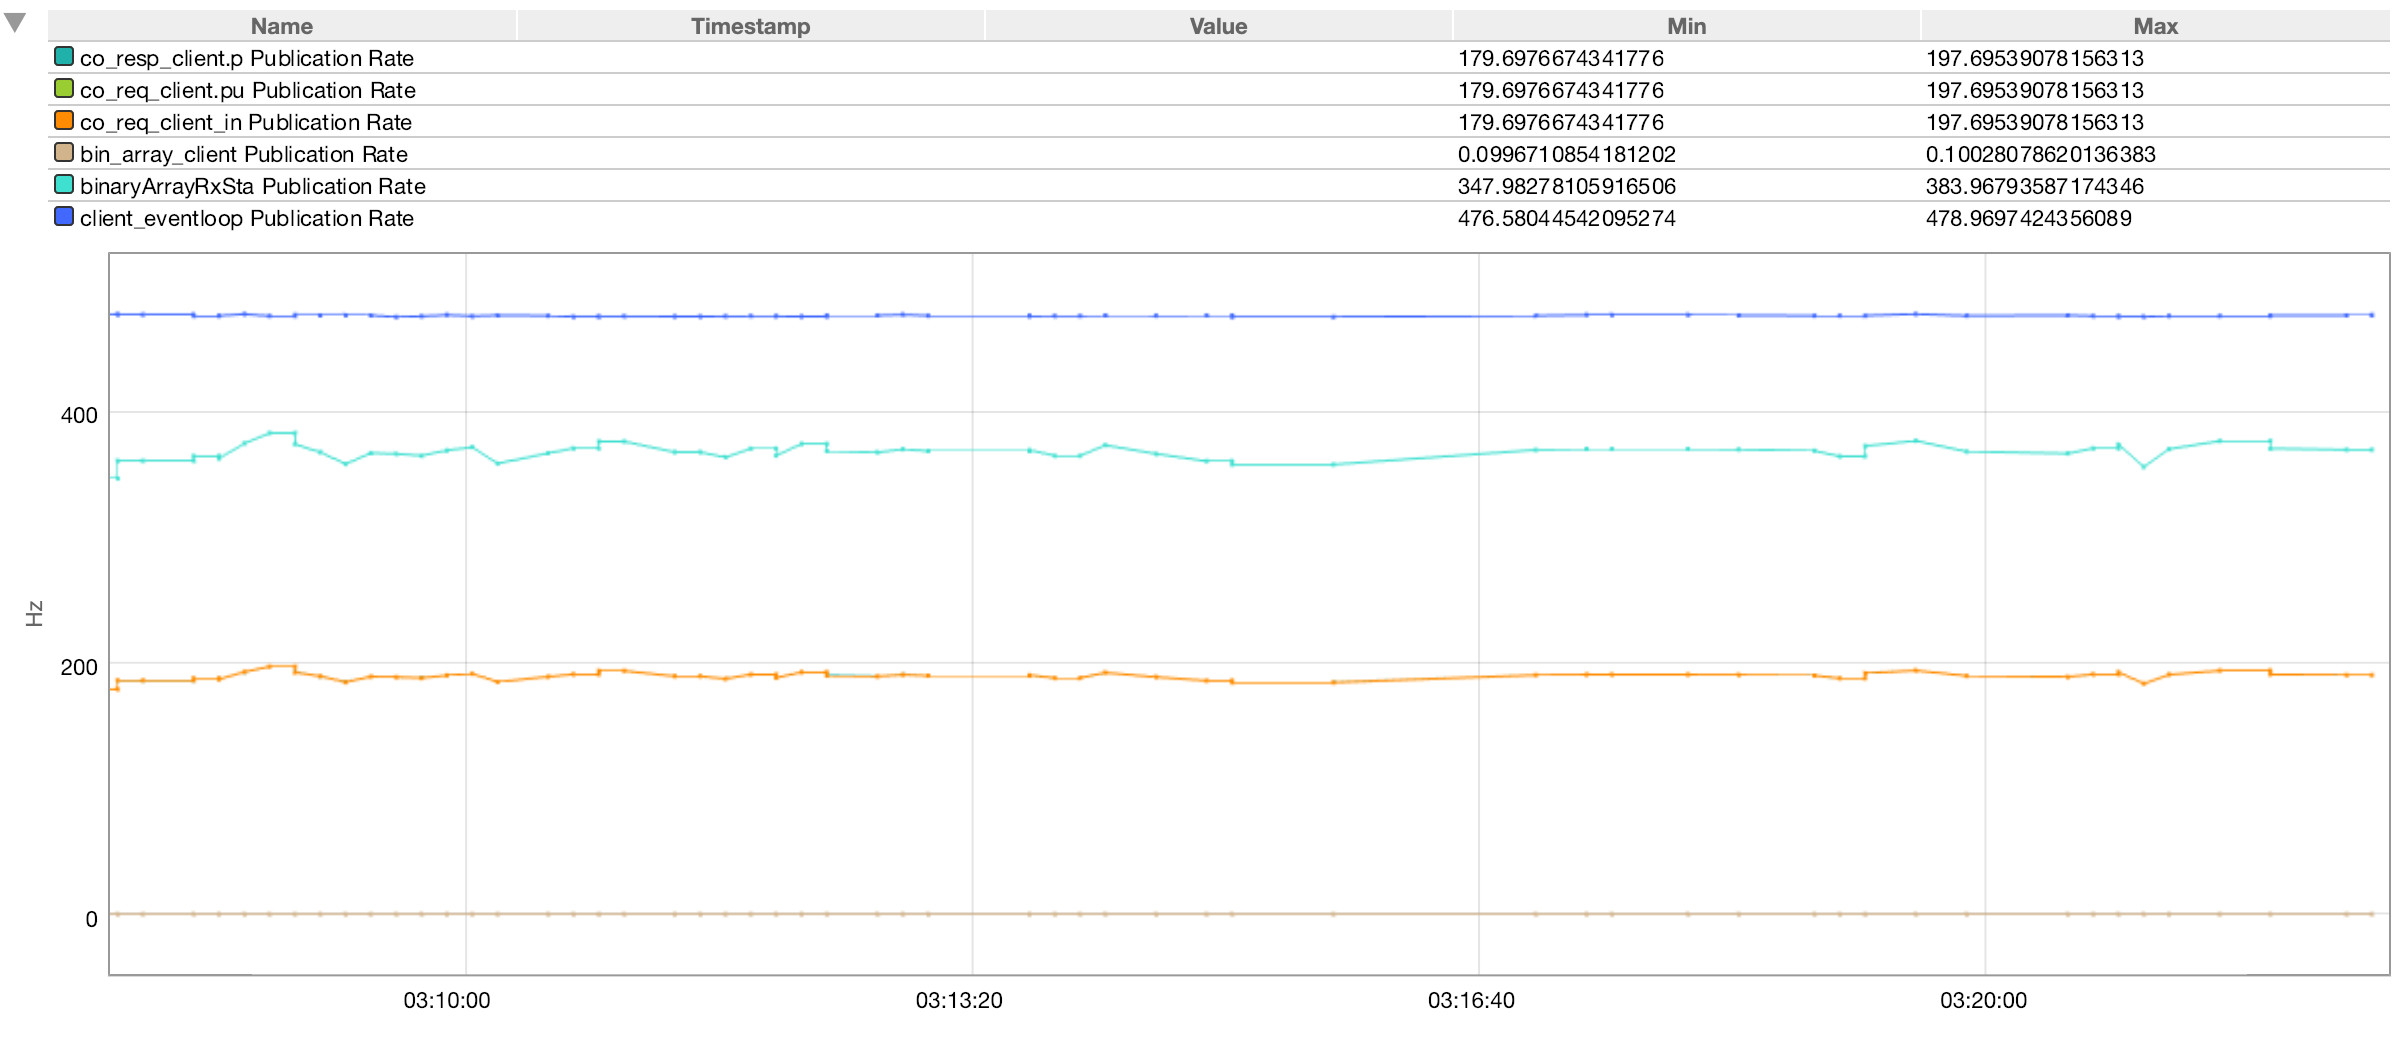
\includegraphics[width=0.5\textwidth]{images/client_pub_rate}}
  \subfloat[Client Subscription Rate]{\label{client_subs_rate}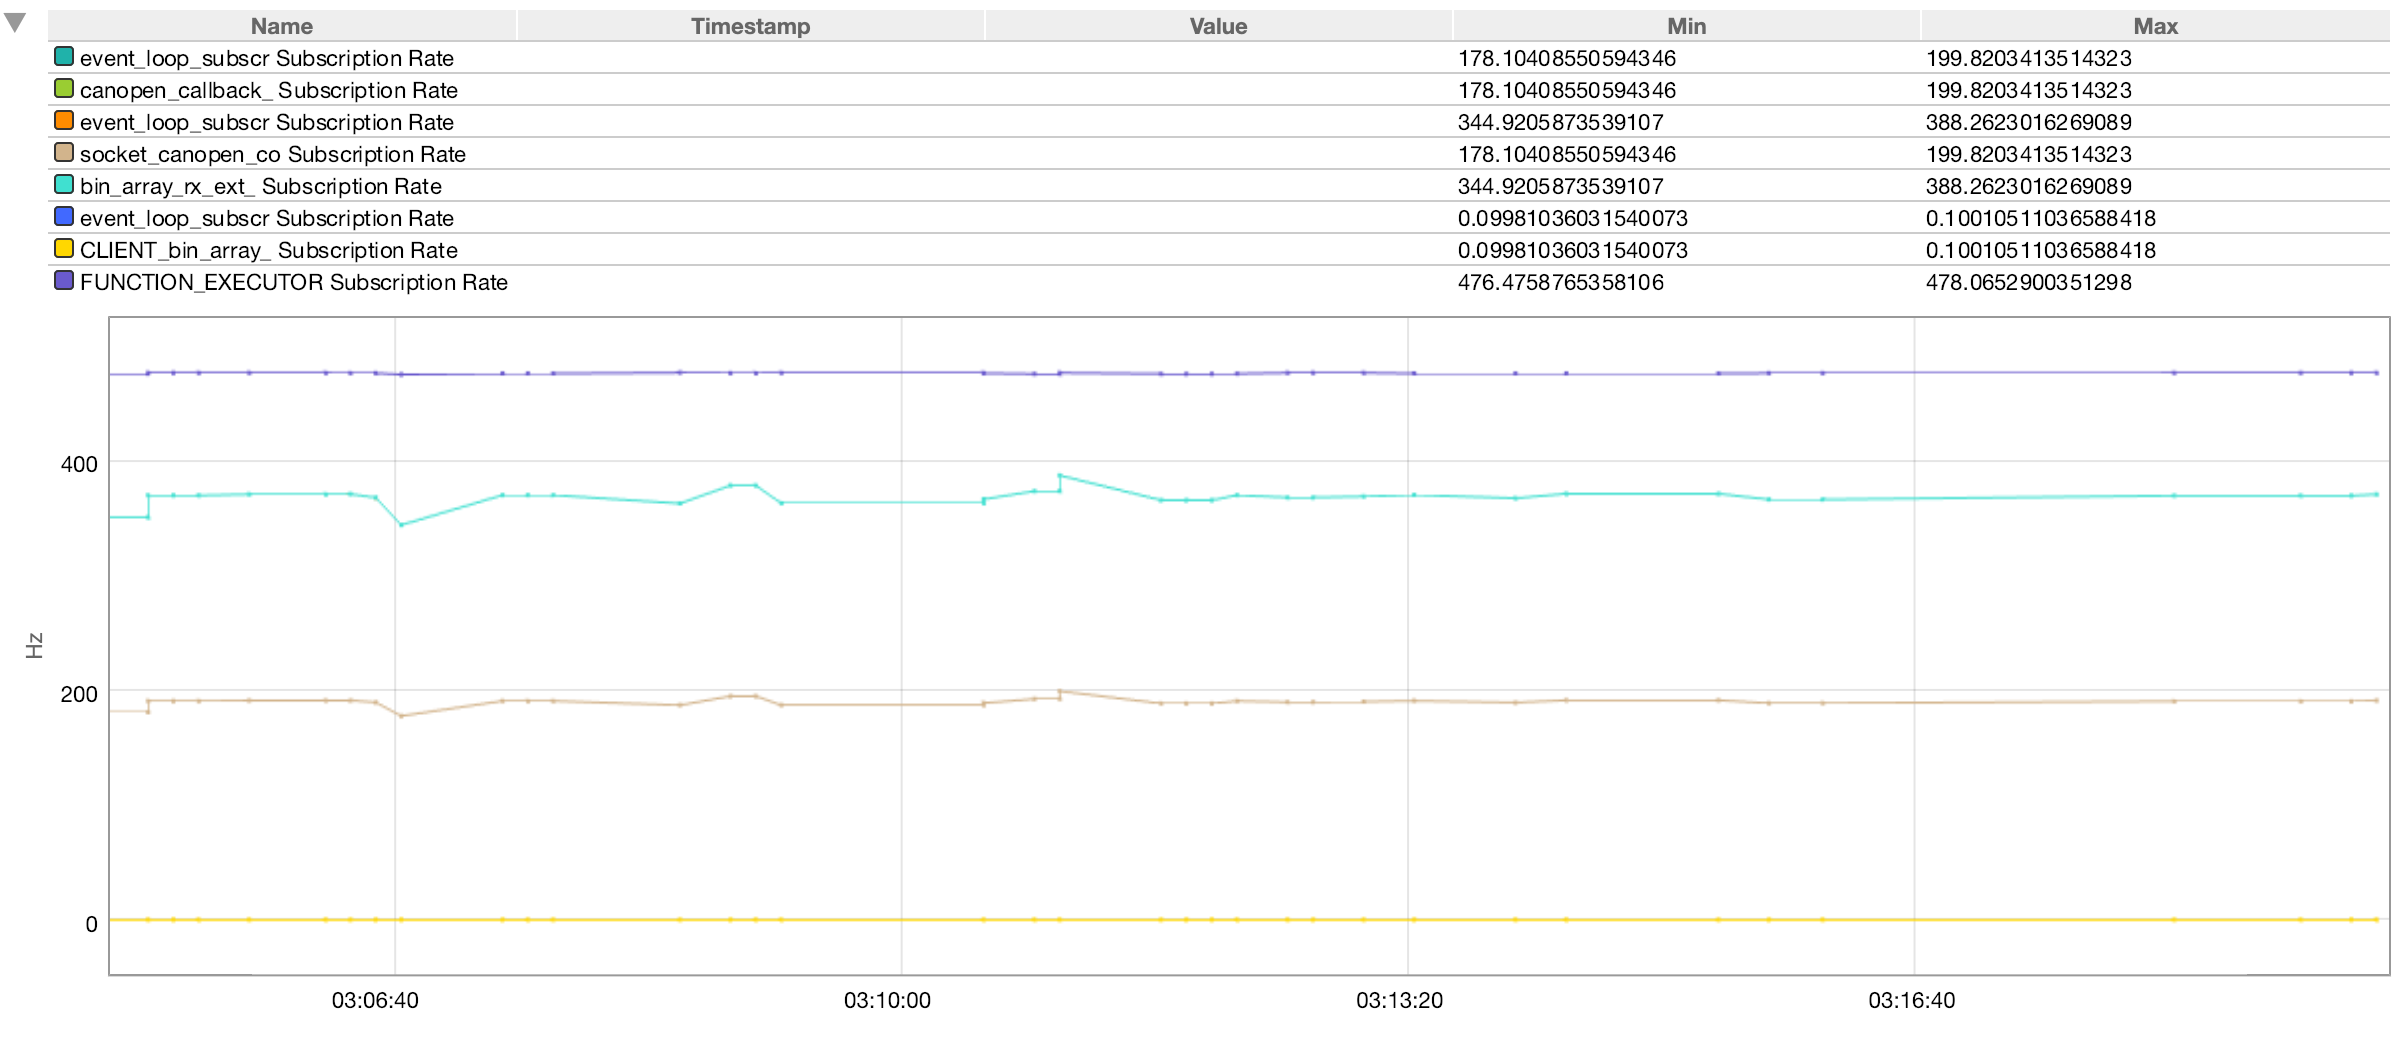
\includegraphics[width=0.5\textwidth]{images/client_subs_rate}}\\
  \subfloat[Server Publication Rate]{\label{server_pub_rate}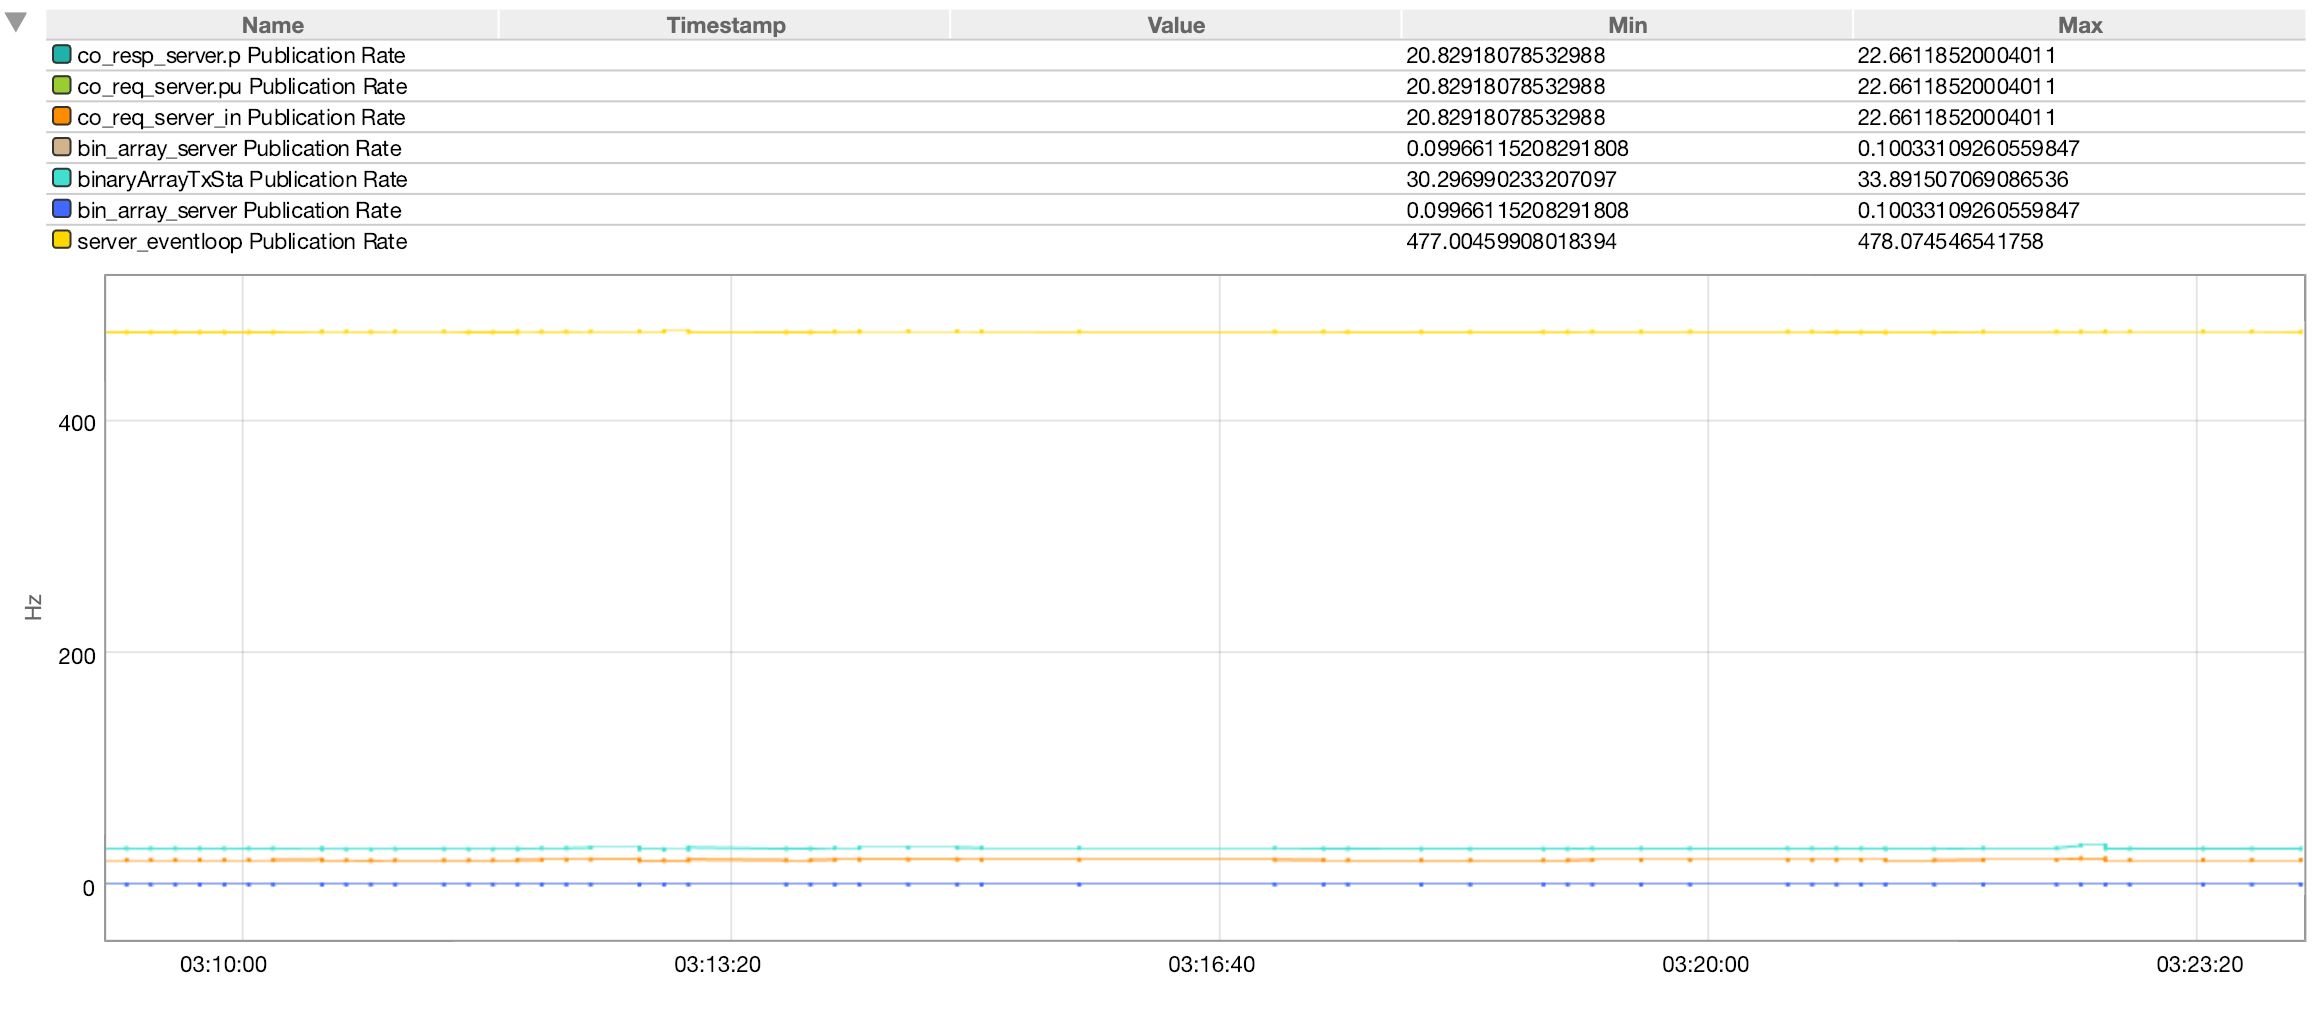
\includegraphics[width=0.5\textwidth]{images/server_pub_rate}}
  \subfloat[Server Subscription Rate]{\label{server_subs_rate}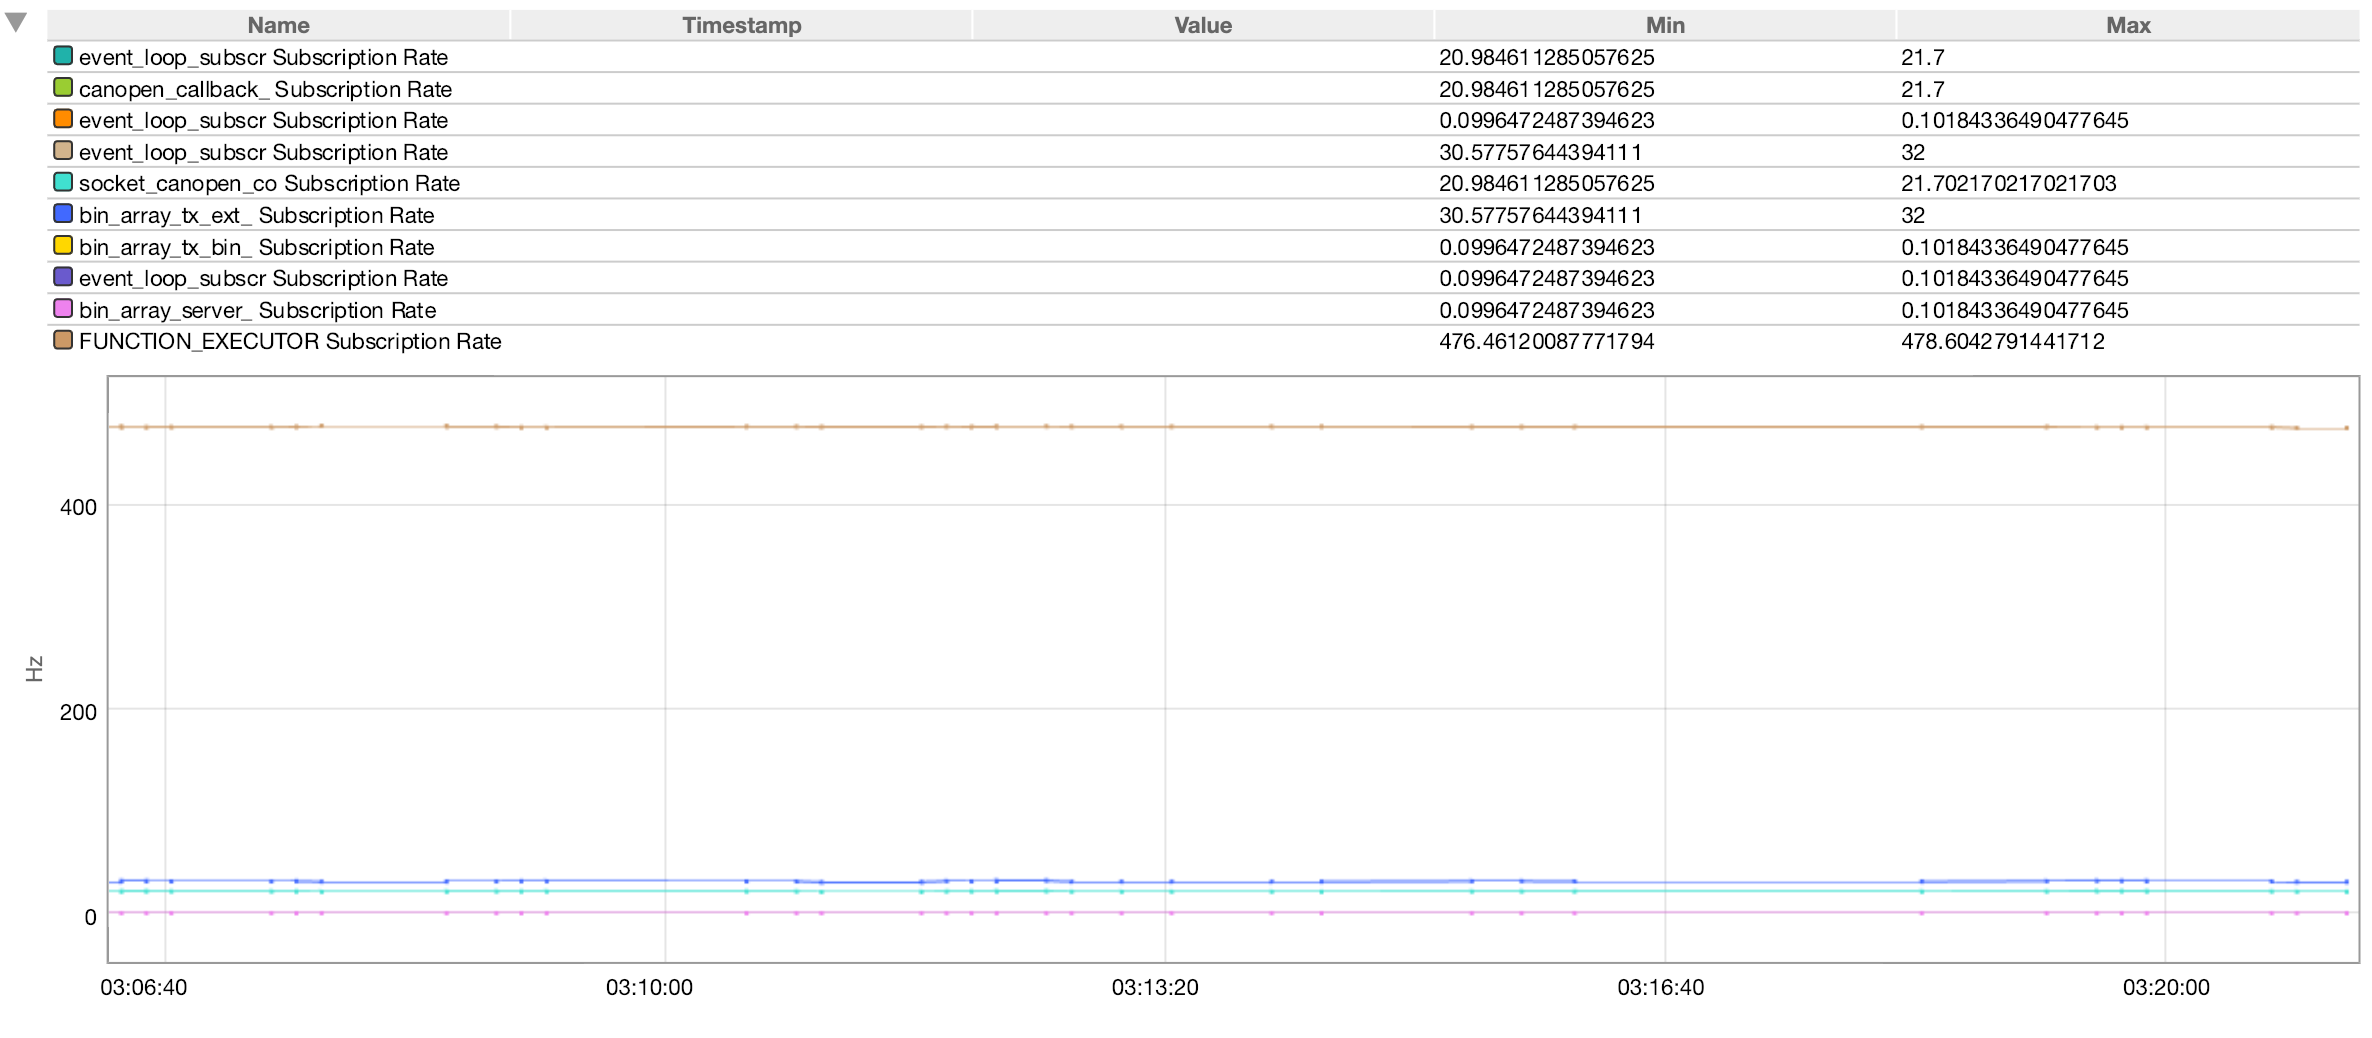
\includegraphics[width=0.5\textwidth]{images/server_subs_rate}}
  \caption{\label{ref_label_overall}Protocol performance}
\end{figure*}

\section{Conclusions}
The Earth Observation solution based on distributed computing using CANopen as middleware presented together by LuxSpace and Klepsydra has shown not only a great throughput, but also stability and predictability that are needed in space conditions. Furthermore, this solution is modular and reusable, making time-to-market in Spacecraft much more attractive and affordable.

\section{Future Work}

Based on the same architectural principles described in this paper, a distributed visual navigation, where the image processing is done in the FPGA, while the host drives the navigation control can provide great benefits to the space community. There are already some works done in the field (\cite{VIS_NAV1}, \cite{VIS_NAV2}, \cite{VIS_NAV3}), which are the base for further work in the field. In that sense, Klepsydra can help providing the optimisation and stability required for such a complex systems. LuxSpace has opted to continue with the development of microsatellites using CAN Networks and CANopen for spacecraft on-board communications and control. However, it is also desired to continue extending the use of the CANopen standard by enhancing the application layer protocol that operates in conjunction with the CAN Network data link layer providing a set of rich services and protocols useful to every device on the network. LuxSpace is currently developing its Triton-X platform, and evolution of the E-SAIL satellite, with 50 kg platform plus 30kg of payload. Triton-X is a satellite-based product line, designed with a high level of flexibility, which allows easy adaptation to different payloads and mission profiles (Earth observation, Space Situational Awareness (SAA), Communication In-orbit Test, Machine-to-machine (M2M) systems and for payload technology demonstration.), minimizing the associated non-recurring engineering cost.

\begin{figure}[H]
\centering
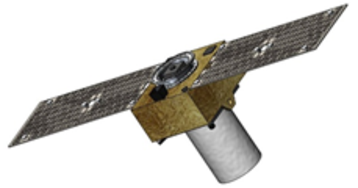
\includegraphics[width = 3in]{images/tritonx}
\caption{\label{fig:tritonx} Triton-X EO design}
\end{figure}

The Triton-X bus will be based on CANopen and it is expected that fast integration of CAN compliant instrumentation will be needed to support the different client requirements. Is in here, where the presence of a software that isolates the low level drivers and protocols complexity such as Klepsydra could be of special benefit, bending the software development to focus on the application layer, enriching the functionality desired by the customers rather than in the problematic of the low level underworld. The first flight of a Triton-X satellite platform is scheduled for 2020.

\FloatBarrier
\bibliography{references/obdp2019} 

\end{document}

